\section{Overview}

The \textbf{Advance Encryption Standard (AES)}, also known as the Rijndael, is the most widely used symmetric cipher today.
It is mandated by several industry standards and incorporated into numerous commercial systems. 
Examples include the Wi-Fi encryption standard IEEE 802.11i, the secure shell network protocol SSH (Secure Shell), and numerous security products around the world. 

AES was developed to replace Data Encryption Standard (DES), becoming the new standard for encryption.
% DES is known to not be very efficient for software implementions and it uses a short block size of 64 bits, which is a drawback in certain applications. 
% For example, building a hash function from a block cipher. 


\subsection{General Structure of AES}

AES operates on 128-bit blocks of data, referred to as the state of the algorithm.
It processes these blocks in several rounds, with each round consisting of multiple layers that manipulate the data in specific ways. 
These layers introduce both \textit{confusion} and \textit{diffusion} to strengthen the encryption.

The AES structure consists of the following layers:
\begin{enumerate}
    \item \textbf{Key Addition Layer}:
    A 128-bit round key is XORed with the state. 
    % This adds the key information to the data at each round. 

    \item \textbf{Byte Substitution Layer (S-Box)}:
    Each byte of the state is non-linearly transformed using lookup tables. 
    This introduces confusion, ensuring that small changes in the input lead to significant, non-linear changes in the output.
    
    \item \textbf{Diffusion Layer}:
    This layer spreads the influence of each byte over the entire block. 
    It is divided into two sub-layers:
    \begin{enumerate}
        \item \textbf{ShiftRow Layer}: The rows of the state are shifted cyclically, which helps spread the data. %permutes the data on a byte level
        \item \textbf{MixColumn Layer}: : This layer performs a matrix multiplication operation on the columns of the state, mixing the data across the block. % is a matrix operation which combines/mixes blocks of four bytes. 
    \end{enumerate}
\end{enumerate}

Each round, except the first, consists of all three layers. 
The final round omits the \textsc{MixColumn} transformation, making both encryption and decryption operations symmetric.

Figure \ref{fig:aes-block-diagram} shows the block diagram of AES encryption.

\begin{figure}[h] % 'h' means place the figure here if possible
    \centering
    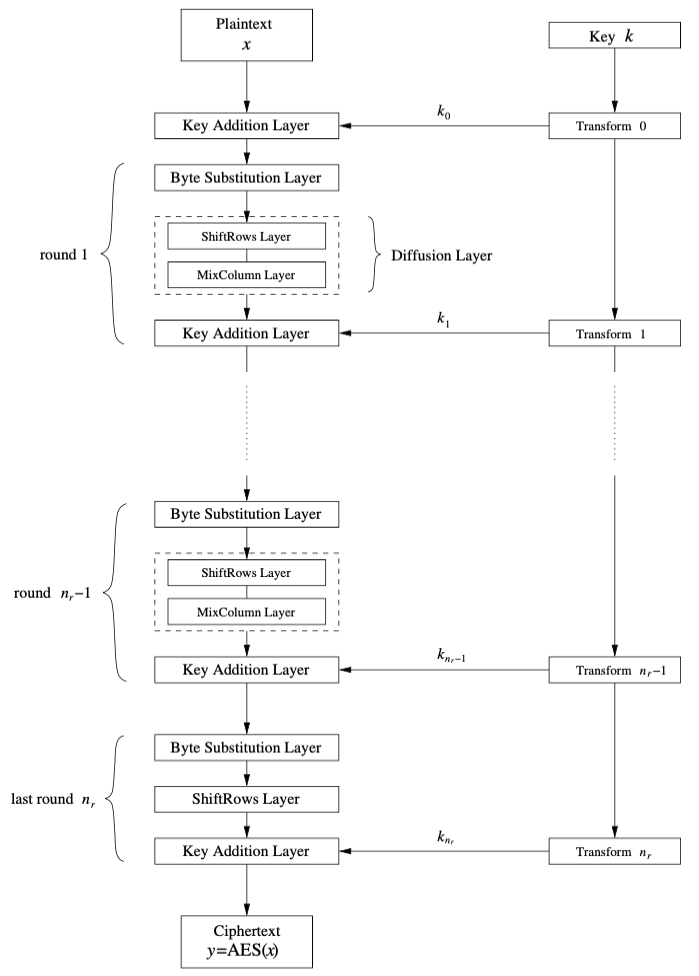
\includegraphics[width=.8\textwidth]{aes-block-diagram.png} % Adjust width as needed
    \caption{
        AES Encryption Block Diagram.
        The plaintext is denoted as $x$, the ciphertext as $y$, key as $k$, and the number of rounds as $n_r$.
    }
    \label{fig:aes-block-diagram} % Reference this figure with \ref{fig:sample_image}
\end{figure}
 


\subsection{Key Size vs. Rounds}

The Rijndeal block and key size vary between 128, 192, and 256 bits.
However, the AES standard calls for a block size of 128 bits. 
The key length directly determines the number of encryption rounds the algorithm performs, as described in 

In AES, the block size is fixed at 128 bits, but the key size can vary between 128, 192, and 256 bits. 
The key length determines the number of rounds used in the encryption process, as outlined in Table \ref{table:key-length-rounds}.

\begin{table}[h]
    \centering
    \begin{tabular}{c|c}
        \textbf{Key length (bit)} & \textbf{\# rounds ($n_r$)} \\ 
        \hline
        128 & 10 \\  
        192 & 12 \\  
        256 & 14 \\  
    \end{tabular}
    \caption{Key lengths and number of rounds for AES}
    \label{table:key-length-rounds}
\end{table}



\subsection{Advantages over DES}

AES offers several advantages over the older DES, particularly in terms of security and efficiency \cite{techtarget_AES_DES}.

\paragraph{Security} 
AES uses a 128-bit block size, compared to DES's 64-bit block size. 
This larger block size significantly enhances security by increasing resistance against brute-force and cryptanalytic attacks. 
% Additionally, AES supports longer key lengths (128, 192, and 256 bits), further improving its cryptographic strength.

\paragraph{Flexibility}
AES supports three different key sizes: 128, 192, and 256 bits, allowing users to choose the level of security they need based on their specific application. 
In contrast, DES uses a fixed 56-bit key, which limits its cryptographic strength. 
Developers can choose from multiple key lengths in AES allows for greater adaptability in meeting varying security requirements.%, especially as computational power increases over time.

\paragraph{Efficiency}
AES processes all 128 bits of data in each round, whereas DES effectively operates on 32 bits per round due to its Feistel structure, which splits the 64-bit block into two halves. 
This allows AES to achieve a higher throughput with fewer computational steps, making it well-suited for both software and hardware implementations.
